\documentclass[11pt,compress,serif]{beamer}
%\includeonlyframes{current}

\usepackage[utf8x]{inputenc}
\usepackage[T1]{fontenc}
\usepackage[english]{babel}
% \usepackage{booktabs}
\usepackage{hyperref}
\usepackage{url}
%\usepackage{auto-pst-pdf}
%\usepackage{pst-plot}

% \usepackage{pstricks-add}

\usepackage{graphicx}
\definecolor{mygreen}{HTML}{4A7023}

\usepackage{xspace}
\usepackage{xcolor}
\usepackage{minted}
\definecolor{rulecolor}{rgb}{0.80,0.80,0.80}
\newminted{python}{fontsize=\footnotesize}

\graphicspath{{./images/}}


% Theme
\mode<presentation>
{
    \usetheme{default}
}

%\setbeamertemplate{footline}


% Non navigation symbal
\setbeamertemplate{navigation symbols}{}

% Between section
\AtBeginSection[]
{
    %   \frame
    %   {
    %       \frametitle{Outline}
    %       \tableofcontents[currentsection]
    %   }
}

% Between subsection
\AtBeginSubsection[]
{
    %   \begin{frame}<beamer>
    %    \frametitle{Outline}
    %    \tableofcontents[currentsection,currentsubsection]
    %   \end{frame}
}


% Talk information
\author[A. Joly]{\textbf{Arnaud Joly}}
\title{\textbf{The genesis of clusterlib \\An open source library to tame your favourite supercomputer}}
% \institute[Ulg]{\includegraphics[height=2cm]{logo_coul_texte_blason_cadre}}
\date{\textbf{May 2015, Phd hour discussions}}
\subject{}
%\logo{} %change here. I used an eps file logo, you can use jpg or other format


\begin{document}
    
%\frame[plain]
%{
%    \titlepage
%}

{
    \usebackgroundtemplate{
        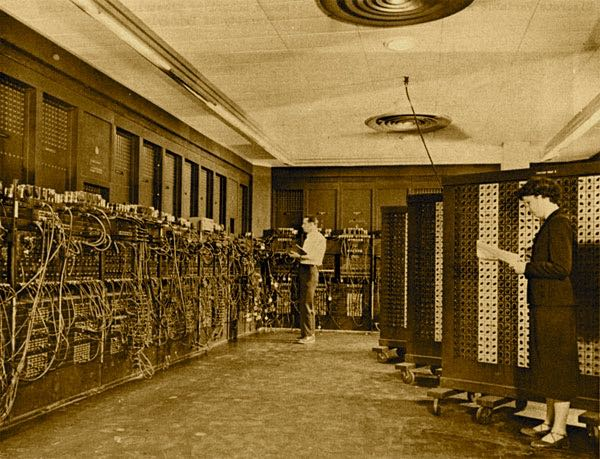
\includegraphics[width=1.0\paperwidth,
        height=1.0\paperheight]{supercomputer-7}}
    \setbeamercolor{title}{fg=white}
    \setbeamercolor{author}{fg=white}
    \setbeamercolor{date}{fg=white}
    
    \frame[plain]{\titlepage}

%The picture is a public-domain U.S. Army Photo of the ENIAC. All of the wires, switches and components are part of the ENIAC with two of the team of operators helping run the machine. The ENIAC is now being displayed at the Smithsonian Institution in Washington D.C. In 1996, the U.S. Postal Services released a new stamp commemorating the 50th birthday of the ENIAC.




}

\frame{

\frametitle{Use case for the birth of clusterlib}
\framesubtitle{Solving supervised learning tasks}
The goal of supervised learning is to learn a function from
\structure{input}-\alert{output} pairs in order to predict the \alert{output} 
for any new \structure{input}.

\begin{footnotesize}
    \begin{columns}[b]
        \begin{column}{0.5\textwidth}
            \begin{block}{}
                \structure{A supervised learning task}
                
                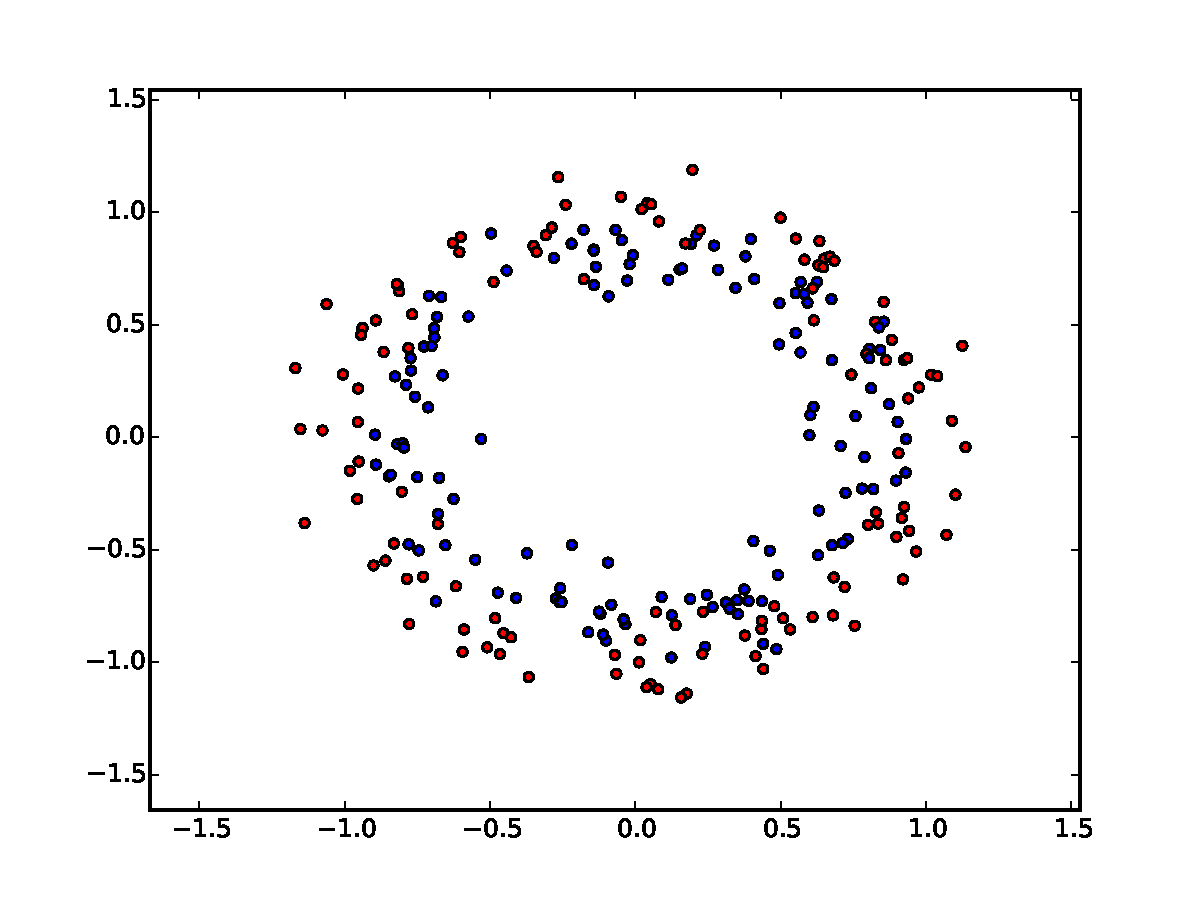
\includegraphics[width=\textwidth]{no_learn}
            \end{block}
        \end{column}
        
        \begin{column}{0.5\textwidth} 
            \structure{A learnt function}               
            
            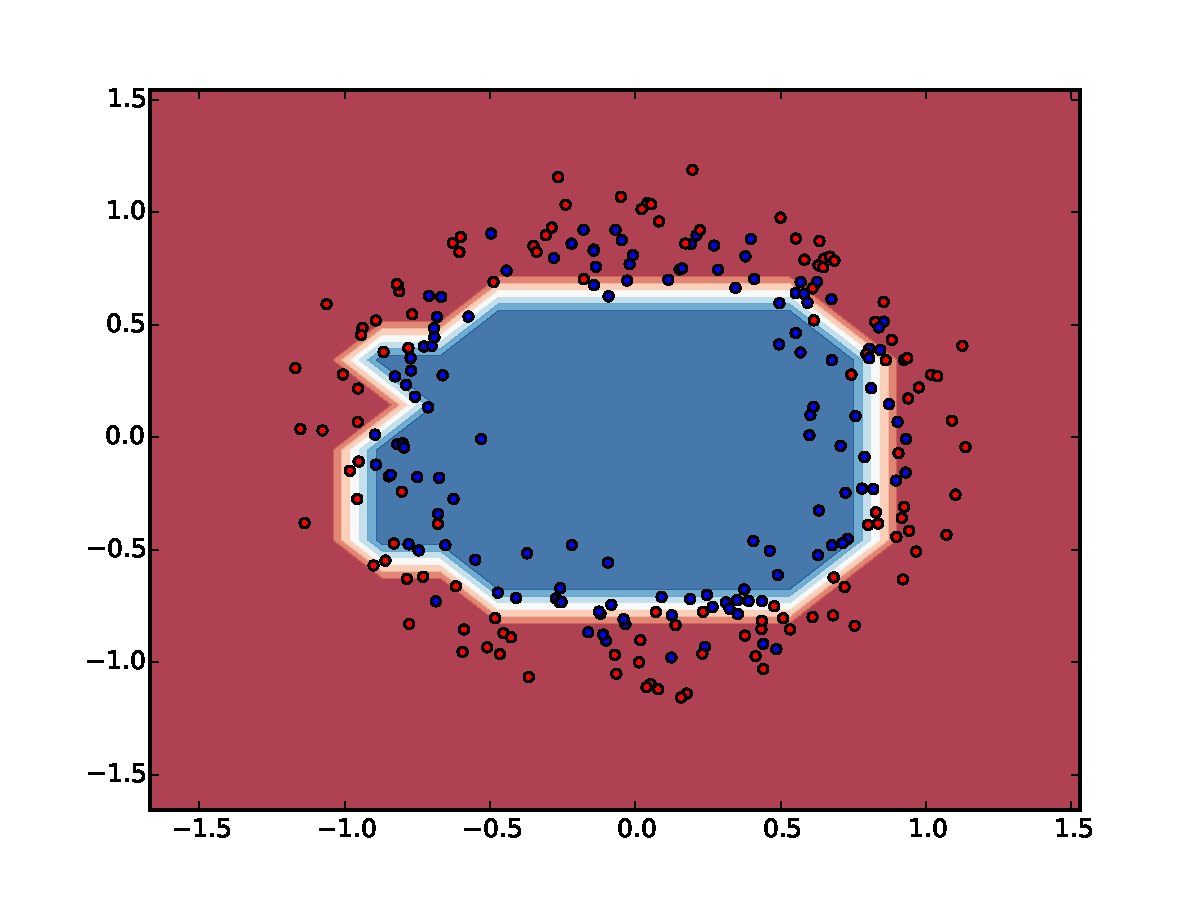
\includegraphics[width=\textwidth]{decision_tree_boundary}
            
        \end{column}
    \end{columns}
\end{footnotesize}
}

%\frame{
%\frametitle{Use case for the birth of clusterlib (II)}
%\framesubtitle{Compression of random forest models}
%The learnt function was a decision tree model. Nowadays instead of only one tree, 
%we generate very large ensemble of randomized decision trees.
%    
%\begin{center}    
%    \includegraphics[width=0.7\textwidth]{decision_tree_structure}
%\end{center}
%
%How to compress those models while preserving accuracy? 
%\emph{L1-based compression of random forest models}
%\cite{joly2012l1}
%}


%\frame{
%\frametitle{Use case for the birth of clusterlib (III)}
%\framesubtitle{Solving high dimensional multilabel classification tasks}
%
%Many applications in text, biology or image processing where samples are associated 
%to sets of labels or continuous response.
%
%\begin{columns}[T]
%    \begin{column}{0.5\textwidth}
%        \begin{block}{Input $\mathcal{X}$ $800 \times 600$ pixel}
%            \begin{center}
%                \includegraphics[width=\textwidth]{image_anotation}
%            \end{center}
%        \end{block}
%    \end{column}
%    
%    \begin{column}{0.4\textwidth}        
%        \begin{block}{Output $\mathcal{Y}$ labels}
%            driver, mountain, road, car, tree, rock, line, human, \ldots
%        \end{block}
%        
%        \begin{block}{}
%            If each label corresponds to a wikipedia article, then we have
%            around \alert{4 million labels}.
%        \end{block}
%    \end{column}
%\end{columns}
%
%How to handle very high label space? \emph{Random forests with random projections of the output space 
%for high dimensional multi-label classification \cite{joly2014random}}
%}

\frame{
\frametitle{Time is running out}

A huge set of tasks and a practical upper bound
\[
O(\text{\#datasets} \times  \text{\#algorithms}  \times  \text{\#parameters}) \leq \text{Time before deadline}
\]
 
\alert{Embarrassingly parallel tasks}.
  
}


\frame{
    \frametitle{Supercomputer = scheduler + workers}
    \framesubtitle{Supercomputer = cluster of computers}    
    
    \begin{center}
        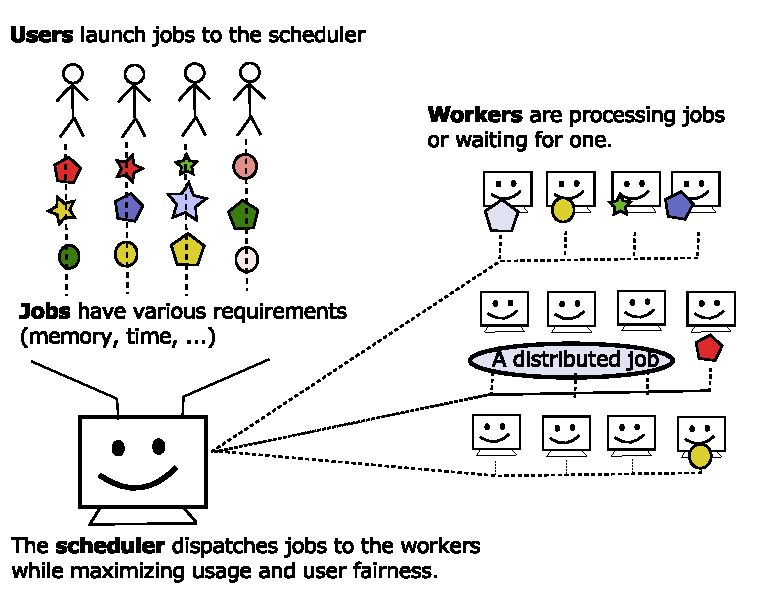
\includegraphics[width=0.9\textwidth]{scheduler}
    \end{center}
    
}

\frame{
\frametitle{CECI is in !}    
Thanks to the CECI\footnote{\emph{The CECI  (\url{http://www.ceci-hpc.be/}) is a supercomputer 
consortium funded by the FNRS.}} at the University 
of Liège, we have access to 

\begin{description}
\item[7] supercomputers (or clusters of computers);
\item[$\approx$ 20 000] cores; % 2048 + 2752 + 896 + 416+  1380 + 816 + 3288 + 8208
% 128 * 64  +  43 * 256 + 32 * 36 +  26 *128 + 115 * 48 + 17 * 128 + 274 * 24 +  342 * 64
\item[>60 000] GB ram;
\item[12] high performance scientific GPU.
\end{description}

}



\begin{frame}[fragile=singleslide]
\frametitle{A glimpse to the SLURM scheduler user interface}
\framesubtitle{How to sumit a job?}

First, we need to write a bash file \texttt{job.sh} which specifies 
resource requirements and calls the program.
\begin{minted}[fonsize=\small]{bash}
#!/bin/bash
#SBATCH --job-name=job-name
#SBATCH --time=10:00
#SBATCH --mem=1000
srun hostname
\end{minted}

\vfill

Then you can launch the job in the queue
\begin{minted}[fonsize=\small]{bash}
$ sbatch job.sh
\end{minted}

\vfill

\alert{How to launch easily many jobs?}

\end{frame}

\begin{frame}[fragile=singleslide]
\frametitle{With clusterlib, how to launch easily many jobs??}

Let's generate jobs submission command on the fly!

\begin{pythoncode}
>>> from clusterlib.scheduler import submit
>>> script = submit(job_command="srun hostname", 
...                 job_name="test",
...                 time="10:00", 
...                 memory=1000, 
...                 backend="slurm")
>>> print(script)
echo '#!/bin/bash
srun hostname' | sbatch --job-name=test --time=10:00 --mem=1000 

>>> # Let's launch the job
>>> os.system(script)
\end{pythoncode}
    
\end{frame}


\begin{frame}[fragile=singleslide]
\frametitle{A glimpse to the SLURM scheduler user interface}
\framesubtitle{How to check if a job is running?}

To check if a job is running, you can use the \texttt{squeue} command.

\begin{minted}{bash}
$ squeue -u `whoami`
\end{minted}

\begin{minted}[fontsize=\scriptsize]{bash}
JOBID   PARTITION     NAME       USER  ST       TIME  NODES NODELIST(REASON)
1225128      defq job-9999    someone  PD       0:00      1 (Priority)
1225129      defq job-9998    someone  PD       0:00      1 (Priority)
...
1224607      defq job-0003    someone   R    7:39:16      1 node025
1224605      defq job-0002    someone   R    7:43:25      1 node040
1224593      defq job-0001    someone   R    8:06:33      1 node035
\end{minted}

\vfill

\alert{How to avoid launching running, queued or completed jobs?}

\end{frame}


\begin{frame}[fragile=singleslide]
\frametitle{With clusterlib, how to avoid re-launching ... ?}

\begin{block}{... running and queued jobs?}
Let's give to jobs a unique name, then let's retrieve
the names of running / queued jobs. 

\begin{pythoncode}
>>> from clusterlib.scheduler import queued_or_running_jobs
>>> queued_or_running_jobs()
["job-0001", "job-0002", ..., "job-9999"]
\end{pythoncode}

\end{block}


\begin{block}{... completed jobs?}
A job must indicate through the file system that it has been completed {\footnotesize e.g. by
creating a file or by registering completion into a database.}

\structure{clusterlib} provides a small NO-SQL database based on sqlite3.
\end{block}

\end{frame}



\begin{frame}[fragile=singleslide]
\frametitle{Simplicity beats complexity}


With only 4 functions

\begin{pythoncode}
from clusterlib.scheduler import queued_or_running_jobs
from clusterlib.scheduler import submit 
from clusterlib.storage import sqlite3_dumps
from clusterlib.storage import sqlite3_loads
\end{pythoncode}

\begin{itemize}
    \item We launch easily thousands of jobs.
    \item We are task DRY (Don't repeat yourself).
    \item We are smoothly working on SLURM and SGE schedulers.
    \item We have only a dependency on python, 
\end{itemize}    

\end{frame}

\frame{
    \begin{center}
        \begin{huge}
            \structure{Are we done?}
            
            \vfill
            
            \visible<2->{Let's go open source!}
        \end{huge}
    \end{center}    
    
}

\frame{
\frametitle{Why making an open source library?}

\begin{block}{Give back to the open source community.}
\begin{center}

\includegraphics[width=0.5\textwidth]{AffiliateLogosFinal_8}

Open source initiative affiliate communities
\end{center}

\end{block}
}

\frame{
    \frametitle{Why making an open source library?}
    \begin{block}{Bug reports are great!}
    \begin{center}
        
\includegraphics[width=0.7\textwidth]{field_of_dreams}
    \end{center}
    \end{block}
}


\begin{frame}[fragile=singleslide]
\frametitle{Why making an open source library?}


\begin{block}{Welcome new contributors !}
\begin{center}

\includegraphics[width=2cm]{contrib_ogrisel}

\includegraphics[width=2cm]{contrib_asutera}

\includegraphics[width=2cm]{contrib_lesteve}

\includegraphics[width=2cm]{contrib_kpetrov}
\end{center}

\begin{small}
From left to right: Olivier Grisel, Antonio Sutera,  
Loic Esteve (no photo) and Konstantin Petrov (no photo).
\end{small}

\end{block}

\end{frame}

\frame{
\frametitle{Why making open source in sciences? Reproducibility!}
    
\begin{center}

\includegraphics[width=0.5\textwidth]{journal-irreproducible-science}
\end{center}
}


\frame{
\frametitle{Be proud of your code}

\begin{center}

\includegraphics[width=\textwidth]{never_be_ashamed_of_your_code}
\end{center}
    
}

\frame{
    \frametitle{Open source way: Host your code publicly}
    
    \begin{center}
    \huge{\structure{www.myproject.com}}

    
\includegraphics[width=0.45\textwidth]{GitHub_Logo}
    
\includegraphics[width=0.45\textwidth]{bitbucket_logo_landing}

    \huge{\structure{Another awesome host platform}}    
    \end{center}
    
    \begin{description}    
    \item[Tip] Sit on the shoulders of a giant!
    
    \item[Bonus] Use a control version system such as git (clusterlib choice), mercurial,\ldots
    \end{description}
}

\frame{

\frametitle{Open source way: Choose a license}



\begin{center}

No license = closed source

\visible<2->{GPL-like license = copyleft}

\visible<3->{BSD / MIT-style license = permissive}


\end{center}

\only<1-3>{\structure{In short}}

\only<1>{You can't use or even read my code.}

\only<2>{You can read / use / share / modify my code, \alert{but} 
         derivatives must retains those rights.}

\only<3>{Do whatever you want with the code, \alert{but} keep my name with it.}

\only<4->{For the sake of \alert{open source}, pick a popular open source license.}

\only<5->{For the sake of \alert{wisdom} or \alert{money}, choose carefully.}

\only<6->{For the sake of \alert{science}, go with BSD / MIT-style license.
        \begin{center}
            \structure{Clusterlib is BSD Licensed.}
        \end{center}
        }
}

\frame{

    \frametitle{Open source way: Start an issue tracker}
 
     An issue tracker allows managing and maintaining a list of issues.
 
    \begin{center}
    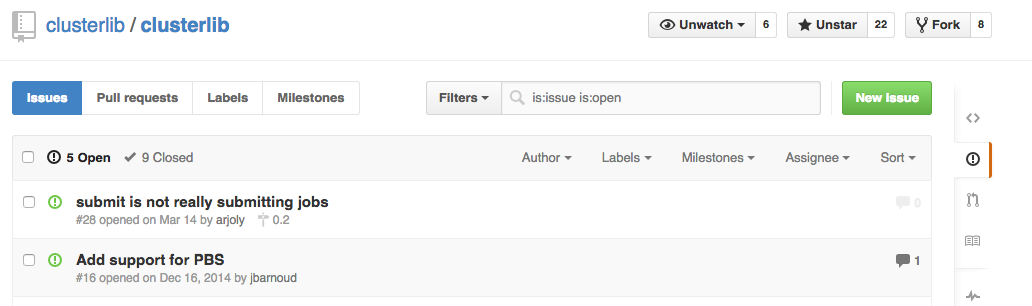
\includegraphics[width=\textwidth]{issue_tracker}
    \end{center}
 
     \begin{description}    
         \item[Tip] Sit on the shoulders of giant\alert{s}! (again) 
     \end{description}       
}

\frame{
     \frametitle{Open source way: Let users discuss with core contributors}   
     
     \begin{enumerate}
     \item Issue tracker (only viable for small project)
     \item Mailing list : sourceforge, google groups, \ldots
     \item Stack overflow tag for big projects
     \end{enumerate}
     
     \vfill
     
     \begin{description}    
         \item[Tip] Sit on the shoulders of giants! (again \alert{* 2}) 
        \end{description}       
}

\frame{
\begin{center}
\begin{huge}
\structure{Are we done?}

\vfill

\visible<2->{The grand  seduction!}
\end{huge}
\end{center}    
    
}

\frame{

\frametitle{Know who you are!}    

\begin{block}{Vision}
The goal of the \structure{clusterlib} is to ease the creation, 
launch and management of embarrassingly parallel jobs 
on supercomputers with schedulers such as SLURM and SGE.    
\end{block}

\vfill

\begin{block}{Core values}
Pure python, simple, user-friendly!
\end{block}

}


\frame{
    \frametitle{Attrative documentation}    
    
    \only<1>{
        \begin{block}{Readme}
        \begin{center}
        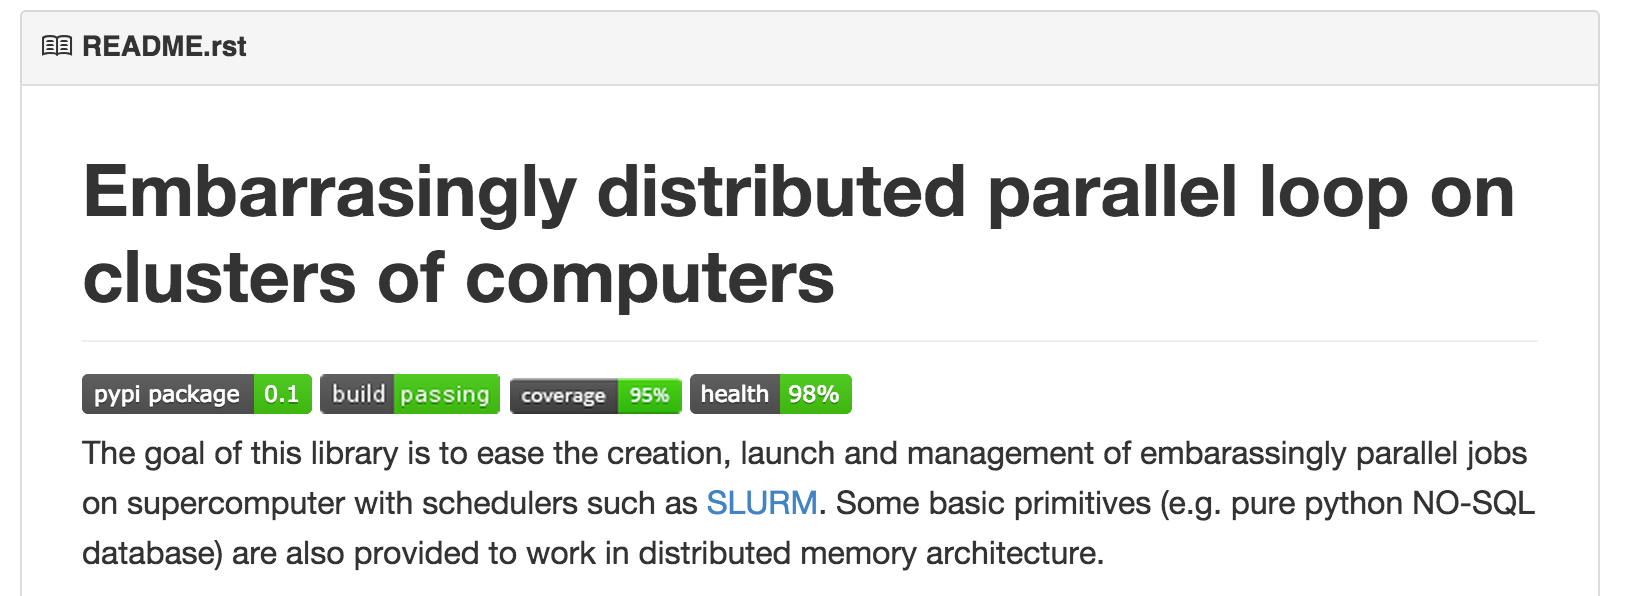
\includegraphics[width=\textwidth]{readme}
        \end{center}
        \end{block}
    }

    \only<2>{
        \begin{block}{API documentation is \structure{nice}.}
            \begin{center}
                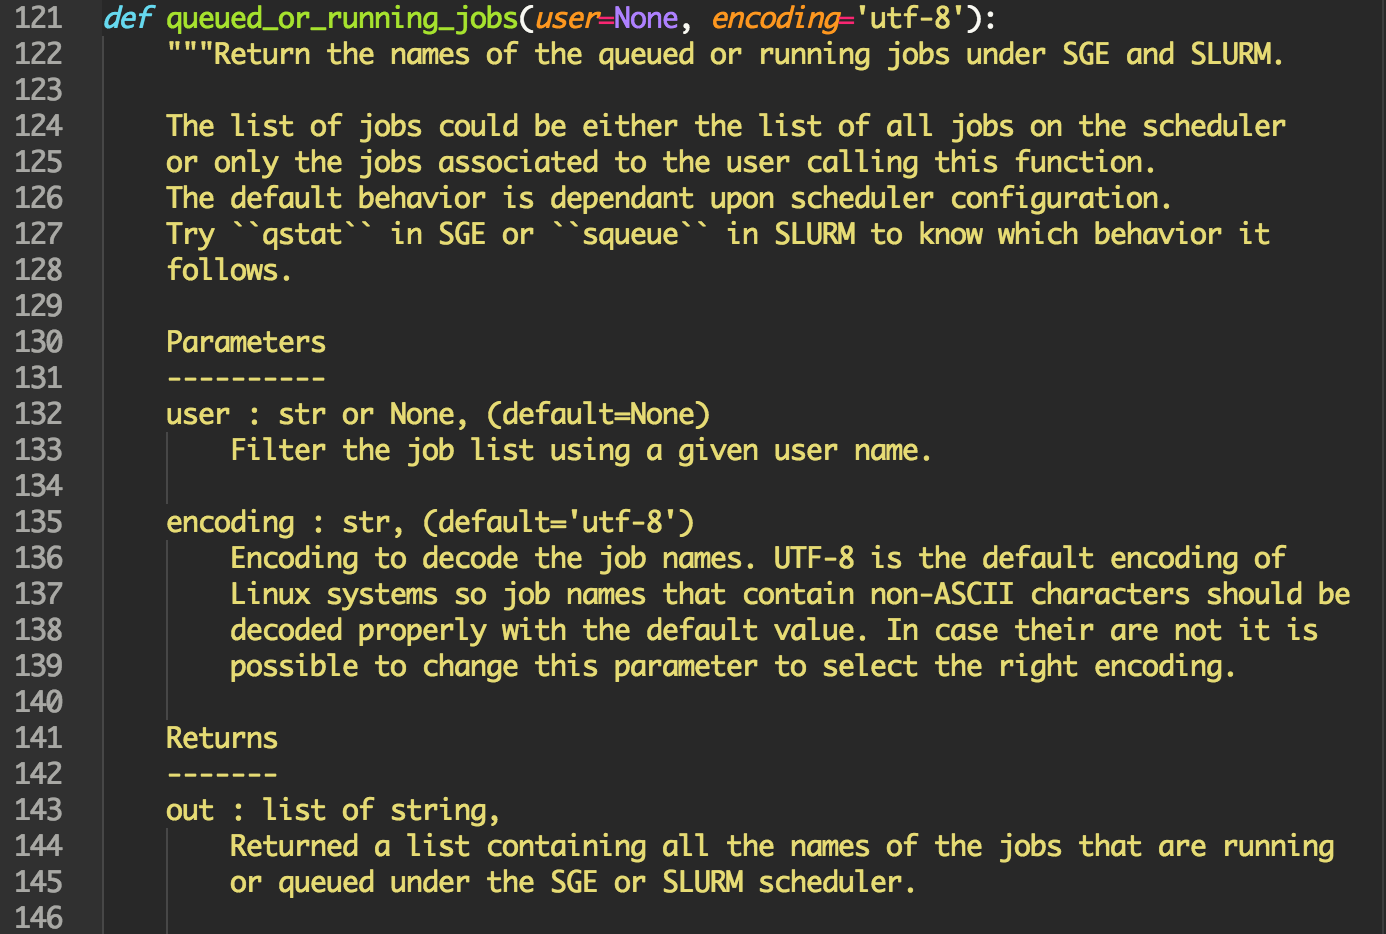
\includegraphics[width=0.7\textwidth]{doc_queued_or_running_job}
            \end{center}
        \end{block}
    
    

        \begin{description}    
%        \item[Tip] Convention >>>>>> configuration! 
%        \item[Tip] Good defaults! 
        \item[Tip] Follow a standard such as "PEP 0257 -- Docstring Conventions".
        \end{description}   
    }
    
    \only<3>{
        \begin{block}{Beautiful doc is \structure{better}.}
            \begin{center}
            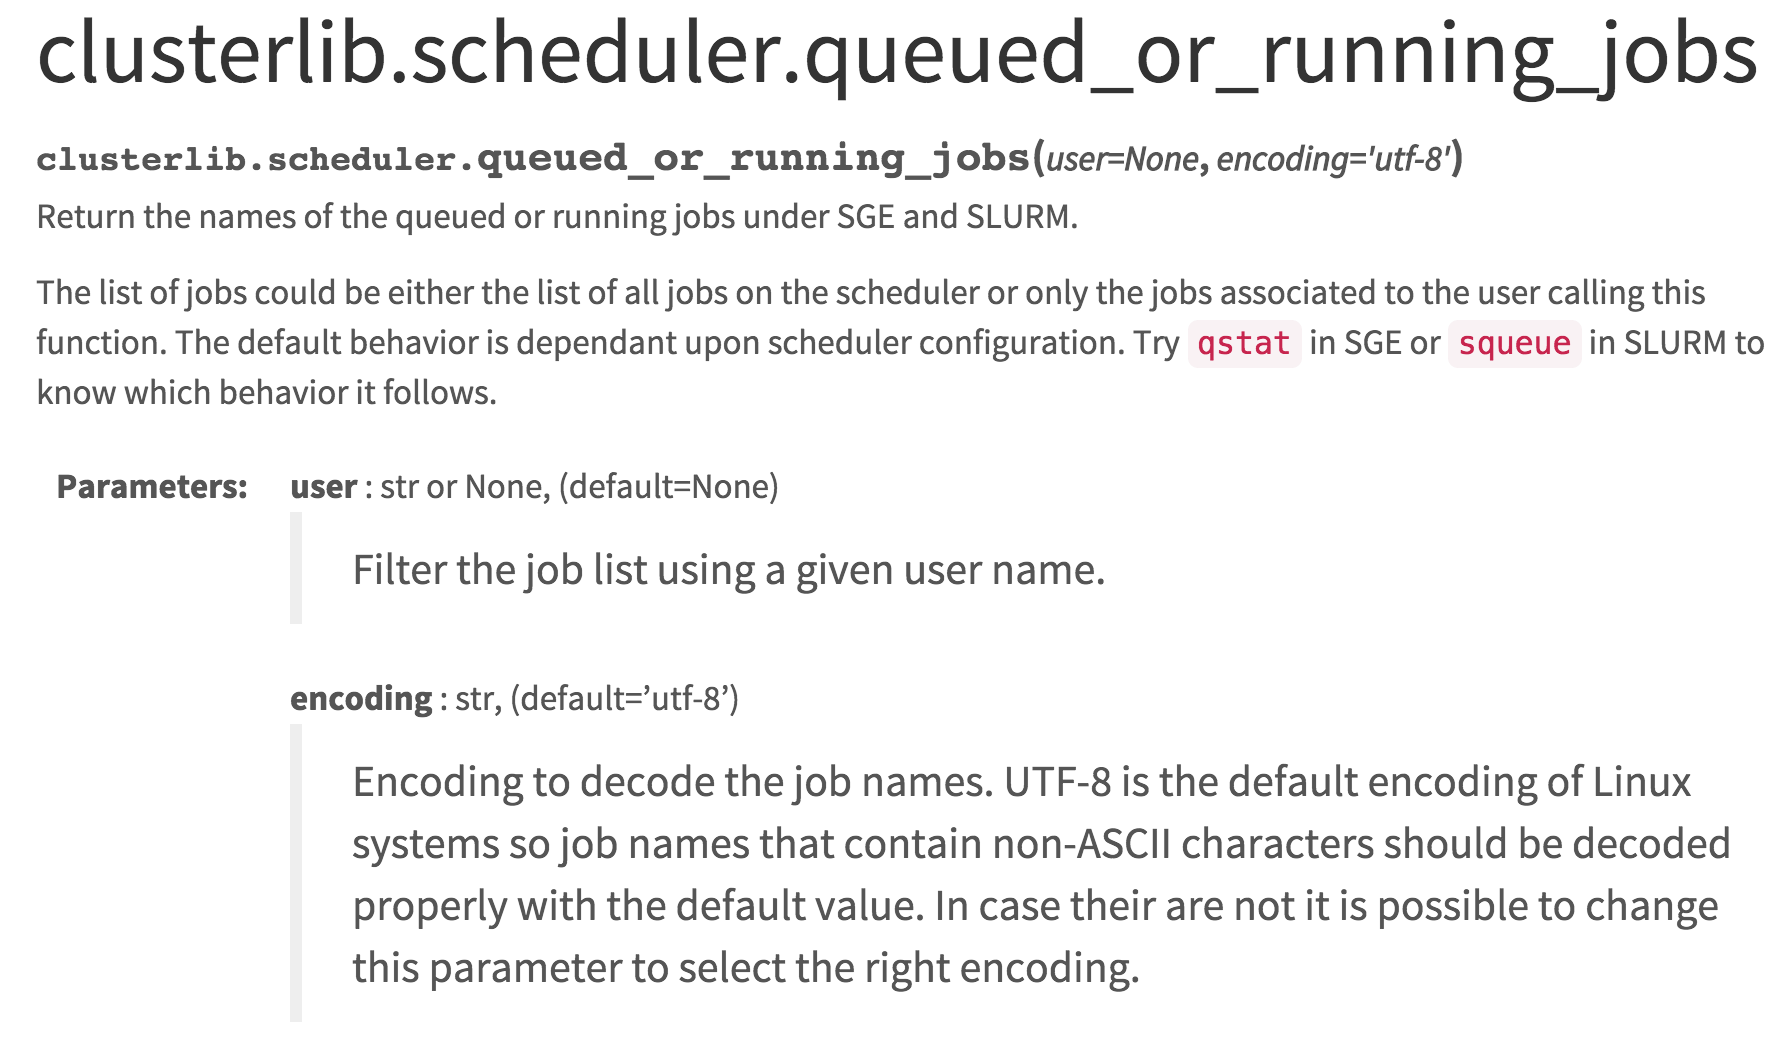
\includegraphics[width=0.9\textwidth]{doc_rendering}
            \end{center}
        \end{block}
    
        \structure{clusterlib} uses sphinx for building its doc. 
    }

    \only<4>{
        \begin{block}{And even better with examples.}
            \begin{center}
                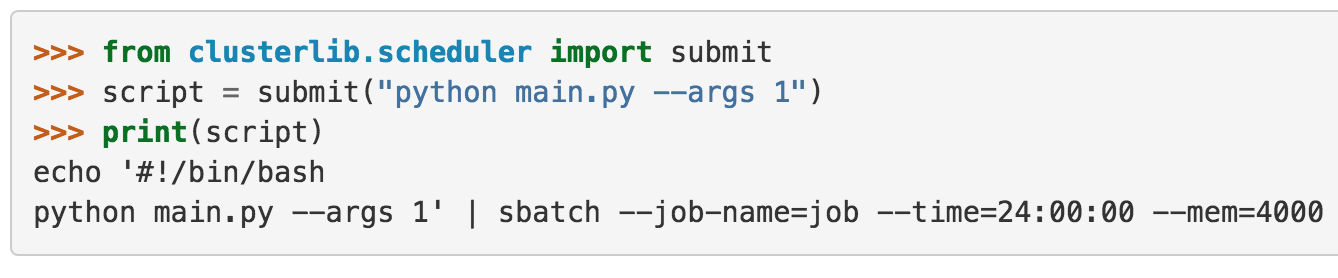
\includegraphics[width=\textwidth]{doc_examples}
            \end{center}
        \end{block}
    }

    \only<5>{
        \begin{block}{A narrative documentation is \structure{awesome}.}
            \begin{center}
                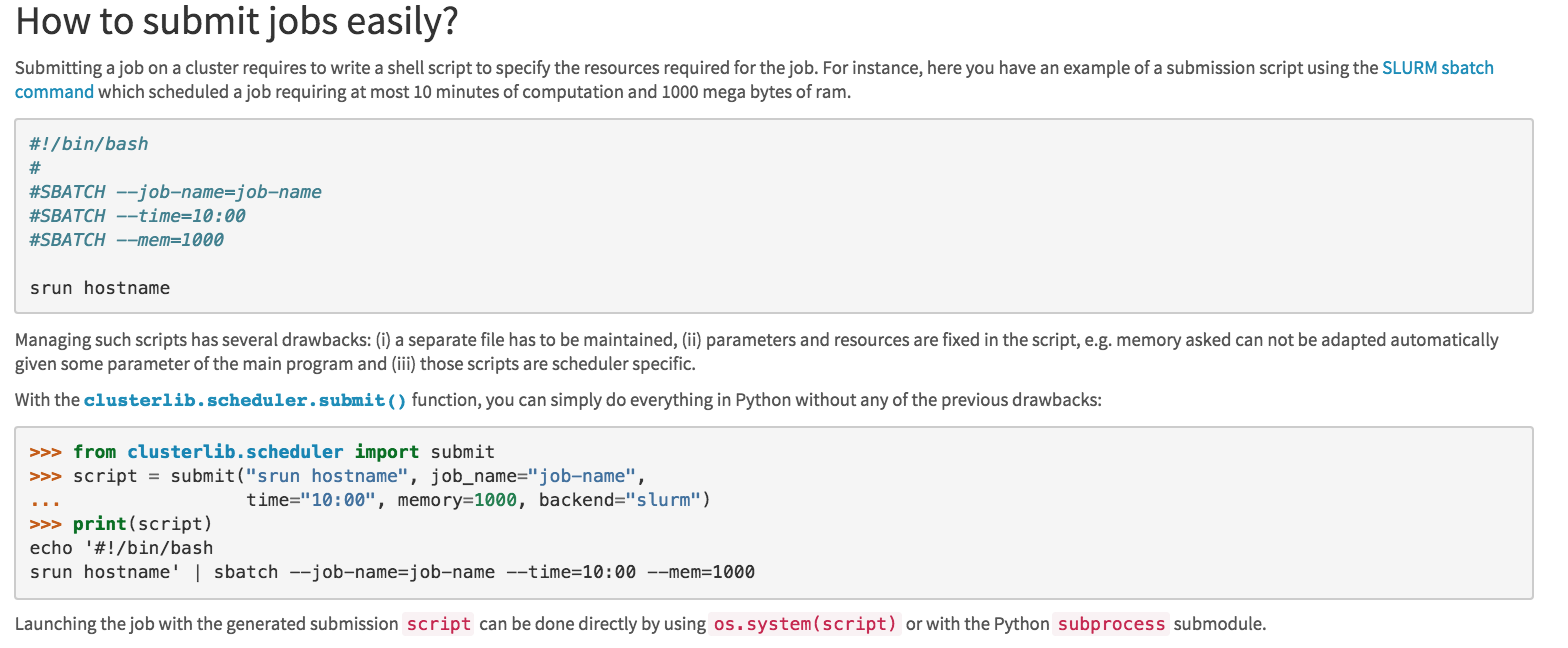
\includegraphics[width=\textwidth]{doc_narrative_documentation}
            \end{center}
        \end{block}
    }
    
    \only<6>{
        \begin{block}{What's new?}
            \begin{center}
                
\includegraphics[width=\textwidth]{doc_whats_new}
            \end{center}
        \end{block}        
        
        Thanks to all clusterlib contributors!
    }
 
}


\begin{frame}[fragile=singleslide]
\frametitle{Appealing test suite}

\structure{How good is your test suite (code coverage)?} 

All code lines are hit by the
tests ($100\%$ line coverage), but not all code paths (branches) are tested.

\begin{minted}[fontsize=\small]{bash}
$ make test 
\end{minted}    
\begin{minted}[fontsize=\scriptsize]{bash}
nosetests clusterlib doc

Name                   Stmts   Miss Branch BrMiss  Cover   Missing
------------------------------------------------------------------
clusterlib                 1      0      0      0   100%   
clusterlib.scheduler      82      0     40     16    87%   
clusterlib.storage        35      0     14      0   100%   
------------------------------------------------------------------
TOTAL                    118      0     54     16    91%   
------------------------------------------------------------------
Ran 12 tests in 0.189s

OK (SKIP=3)
\end{minted}    


\end{frame}

\frame{
    \frametitle{Publicity}    
    
    \begin{center}
        
\includegraphics[width=\textwidth]{publicity_twitter}
    \end{center}
}

\frame{
    \begin{center}
        \begin{huge}
            \structure{Are we done?}
            
            \vfill
            
            \visible<2->{Not yet! Let's make our live easier!}
        \end{huge}
    \end{center}    
    
}

\begin{frame}
    \frametitle{Automation, automation, \ldots}
    
    \only<1>{
        \begin{block}{Continuous testing}
        clusterlib uses \alert{Travis CI} (works for many languages).
                 
        \begin{center}
        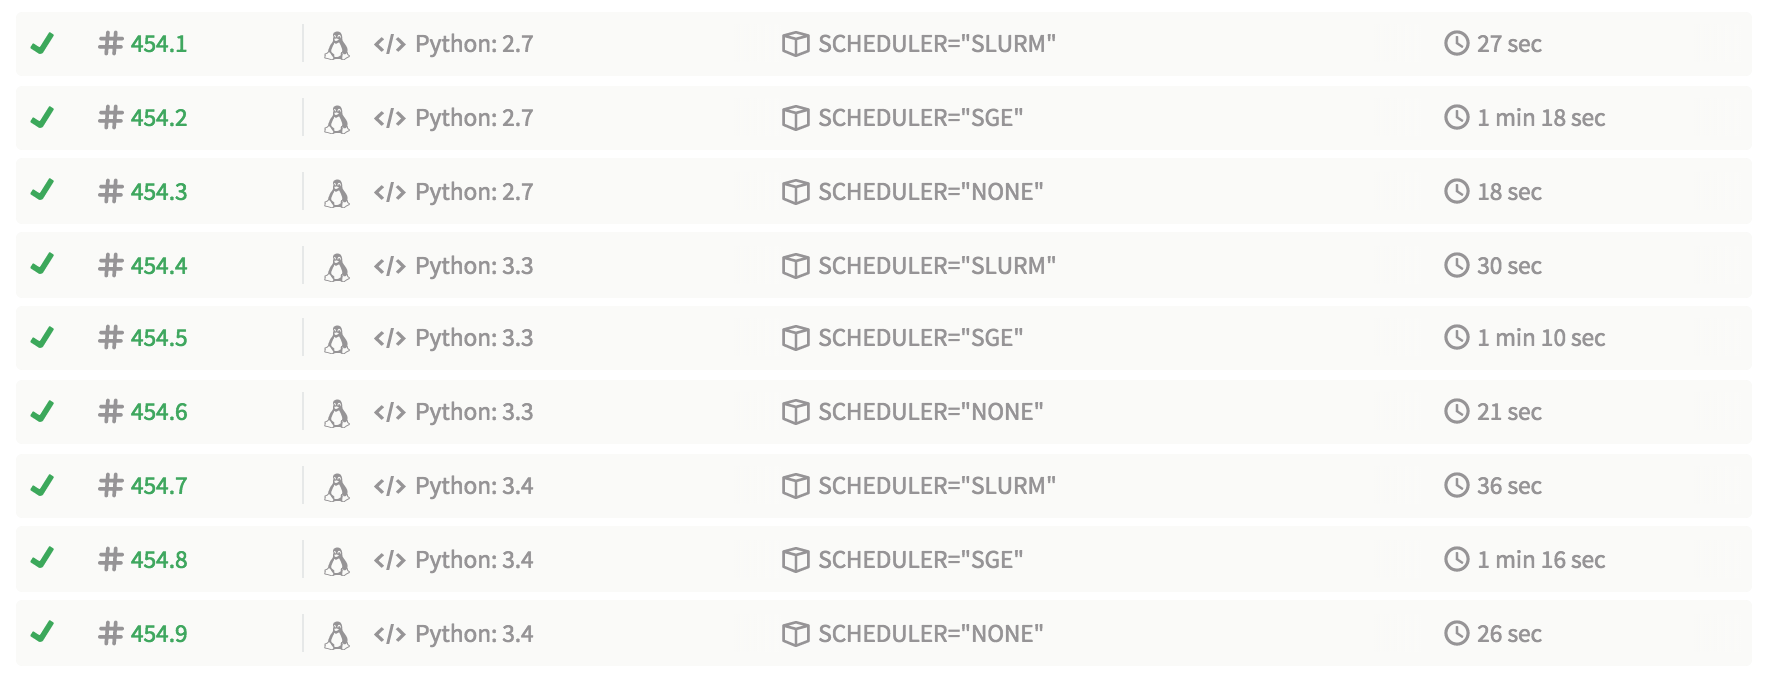
\includegraphics[width=\textwidth]{automation_testing}
        \end{center}

         \begin{description}    
         \item[Tip] Sit on the shoulders of giants! (again \alert{* 3}) 
        \end{description}       
        \end{block}
    }
    
    \only<2>{
        Continuous integration pays off in the long term!        
        
        Ensure test suite is often run. Awesome during development.
        
        \begin{center}
            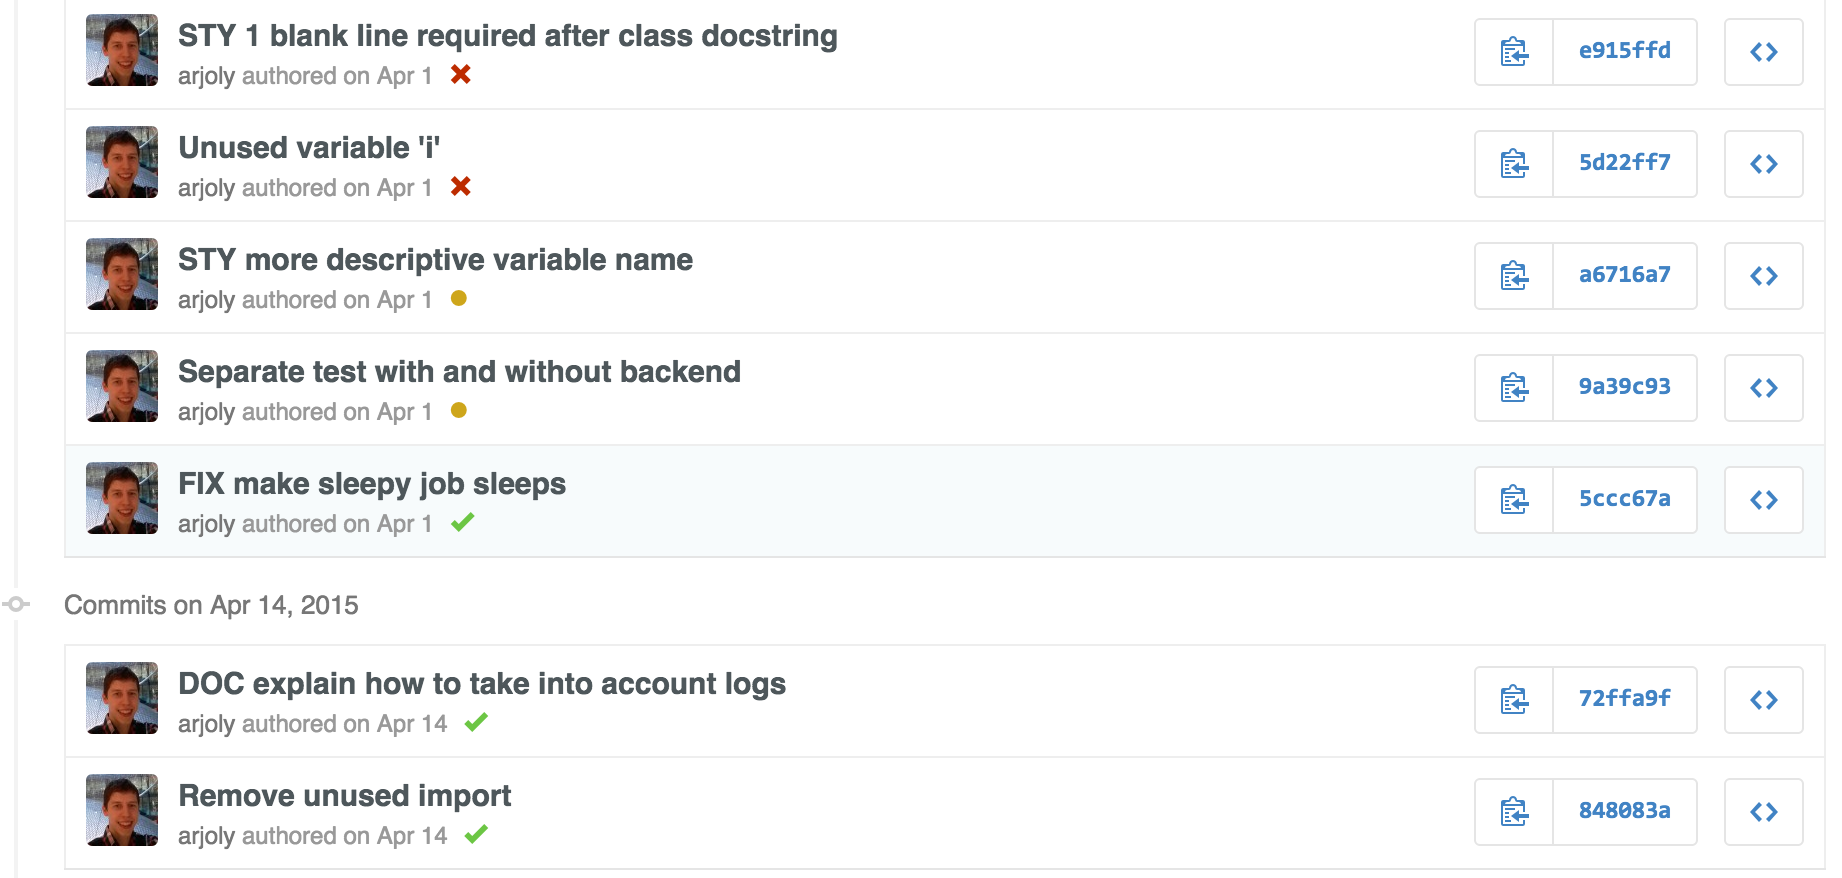
\includegraphics[width=\textwidth]{automate_testing_github}
        \end{center}     
        
         \begin{description}    
             \item[Tip] Continuous integration can be enhanced with code test coverage and code quality coverage. 
         \end{description}          
       
    }

    \only<3>{
        \begin{block}{Continuous doc building}
            
        \begin{center}
            
\includegraphics[width=\textwidth]{automate_doc_building}
        \end{center}    
         
         \begin{description}    
         \item[Tip] Sit on the shoulders of giants! (again \alert{* 4}) 
        \end{description}       
       \end{block}    

     }

\end{frame}

\begin{frame}[fragile=singleslide]
\frametitle{Create and join an open source projects!}

Join a community! Learn the best practices and technologies! 
Make your code survive more than the one project! Give your
code to the world!

\begin{center}
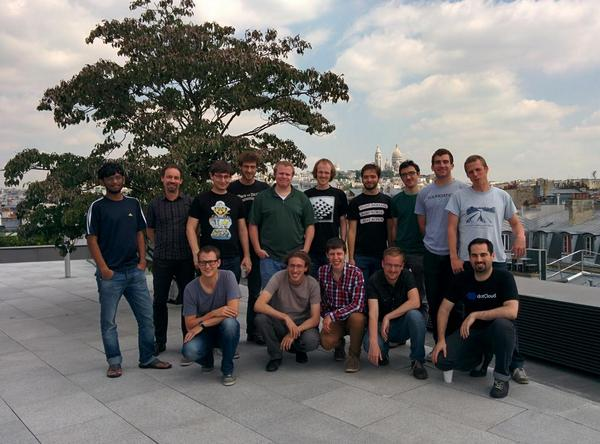
\includegraphics[width=0.7\textwidth]{scikit-learn-sprint.jpg}

\begin{small}
\structure{scikit-learn sprint 2014}
\end{small}
\end{center}

    
\end{frame}




%\frame{
%    \frametitle{Let's not reinvent the wheel}
%    
%    \begin{itemize}
%        \item \structure{Distributed Resource Management Application API} (DRMAA) is a standard api for many 
%        scheduler. Unfortunately, it's not installed by default (installation require root access?).  Some packages are made
%        on top of on this: \structure{python-drma}, \structure{galaxy}, \ldots
%        \item \structure{Bosco} (\url{http://bosco.opensciencegrid.org/}) is a compatibility layer for 
%        several schedulers with similar interface to SLURM/SGE.
%        \item \structure{FireWorks} (\url{http://pythonhosted.org/FireWorks/}) helps run calculation workflows, with a centralized 
%        workflow server controlling many worker nodes. Looks pretty complete, 
%        but much more complex than my basics needs.  6 required dependencies, among 
%        them mongodb, and 7 optional dependencies. 
%    \end{itemize}
%    
%    Arf, \alert{no suitable library} on the market. At this point, I decided to write \structure{clusterlib}.
%    
%}

\begin{frame}[fragile=singleslide]
    \frametitle{A full example of clusterlib usage}
    

\begin{pythoncode}
# main.py

import sys, os
from clusterlib.storage import sqlite3_dumps

NOSQL_PATH = os.path.join(os.environ["HOME"], "job.sqlite3")

def main(argv=None):
    # For ease here, function parameters are sys.argv
    if argv is None: 
        argv = sys.argv  
    # Do heavy computation
    # Save script evaluation on the hard disk

if __name__ == "__main__":
    main()
    # Great, the jobs is done!
    sqlite3_dumps({" ".join(sys.argv): "JOB DONE"}, NOSQL_PATH)
\end{pythoncode}

\end{frame}

\begin{frame}[fragile=singleslide]
    \frametitle{A full example of clusterlib usage}
    
\begin{pythoncode}
# launcher.py
import sys
from clusterlib.scheduler import queued_or_running_jobs
from clusterlib.scheduler import submit
from clusterlib.storage import sqlite3_loads
from main import NOSQL_PATH

if __name__ == "__main__":
    scheduled_jobs = set(queued_or_running_jobs())
    done_jobs = sqlite3_loads(NOSQL_PATH)
    
    for param in range(100):
        job_name = "job-param=%s" % param
        job_command = ("%s main.py --param %s" 
                       % (sys.executable, param))
        if (job_name not in scheduled_jobs and 
                job_command not in done_jobs):
            script = submit(job_command, job_name=job_name)
\end{pythoncode}
    
\end{frame}

\end{document}

